\section{Additional Generalization Diagnostics}

Figure~\ref{fig:appendix-gap} answers two distinct leakage questions using the matched OOF pair pools from RQ4. The upper panel reports, for each HLA locus or H2 restriction, the mean task AUROC change after global peptide separation; zero means no mean change and a negative bar means lower strict performance. The lower panel reports the mean percentage of unique held-out parent proteins that also occur in the fitting partition. A nonzero lower-panel bar therefore shows residual protein identity overlap and demonstrates that peptide-disjoint is not protein-disjoint. The matched standard control is not the original fixed test.

\begin{table}[htbp]
\centering
\caption{Paired task-level standard-versus-strict statistics. Differences are peptide-disjoint OOF minus matched standard OOF. W/T/L counts positive/zero/negative task differences; confidence intervals are 10,000-replicate task-bootstrap intervals for the mean; \(q_{\mathrm{BH}}\) adjusts eight Wilcoxon tests. Splitting the species into panels avoids shrinking the table with \texttt{resizebox}.}
\label{tab:paired-stats}
\small
\setlength{\tabcolsep}{1pt}
\textbf{Human}\par\smallskip
\begin{tabular}{lrrrlll}
\toprule
Metric & Mean & Median & HL & W/T/L & 95\% CI & BH $q$ \\ 
\midrule
AUROC & -0.0628 & -0.0484 & -0.0552 & 12/0/145 & [-0.0728, -0.0534] & $1.29\times10^{-22}$ \\ 
AUPRC & -0.0691 & -0.0509 & -0.0621 & 10/0/147 & [-0.0799, -0.0588] & $1.29\times10^{-22}$ \\ 
Accuracy & -0.0625 & -0.0455 & -0.0563 & 17/2/138 & [-0.0727, -0.0529] & $2.12\times10^{-22}$ \\ 
MCC & -0.1249 & -0.0907 & -0.1125 & 18/0/139 & [-0.1453, -0.1057] & $2.12\times10^{-22}$ \\ 
\bottomrule
\end{tabular}
\par\medskip
\textbf{Mouse}\par\smallskip
\begin{tabular}{lrrrlll}
\toprule
Metric & Mean & Median & HL & W/T/L & 95\% CI & BH $q$ \\ 
\midrule
AUROC & -0.0863 & -0.0832 & -0.0859 & 2/0/22 & [-0.1106, -0.0632] & $6.81\times10^{-7}$ \\ 
AUPRC & -0.0994 & -0.1040 & -0.1002 & 2/0/22 & [-0.1293, -0.0706] & $1.67\times10^{-6}$ \\ 
Accuracy & -0.0918 & -0.0804 & -0.0902 & 1/0/23 & [-0.1207, -0.0652] & $4.77\times10^{-7}$ \\ 
MCC & -0.1838 & -0.1632 & -0.1802 & 1/0/23 & [-0.2415, -0.1306] & $4.77\times10^{-7}$ \\ 
\bottomrule
\end{tabular}
\end{table}

\begin{figure}[htbp]
\centering
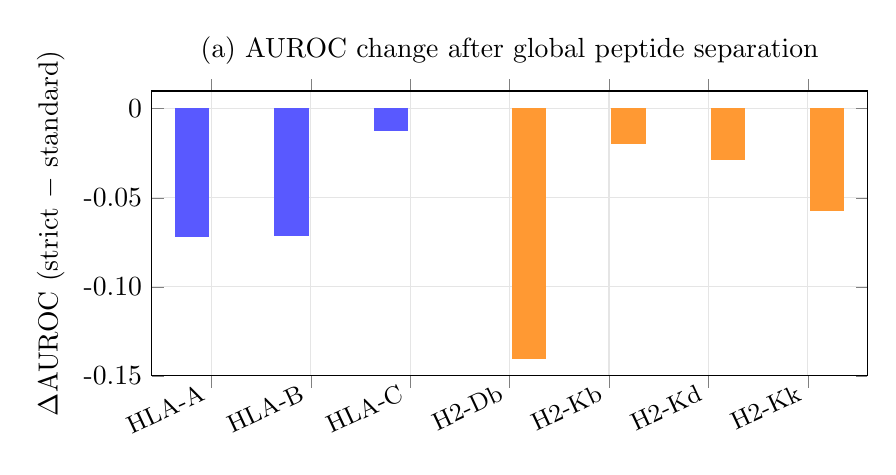
\begin{tikzpicture}
\begin{axis}[
    width=0.88\linewidth,
    height=5.2cm,
    ybar,
    bar width=12pt,
    title={(a) AUROC change after global peptide separation},
    ymin=-0.15,ymax=0.01,
    ytick={-0.15,-0.10,-0.05,0},
    yticklabels={-0.15,-0.10,-0.05,0},
    symbolic x coords={HLA-A,HLA-B,HLA-C,H2-Db,H2-Kb,H2-Kd,H2-Kk},
    xtick={HLA-A,HLA-B,HLA-C,H2-Db,H2-Kb,H2-Kd,H2-Kk},
    x tick label style={rotate=25,anchor=east,font=\small},
    ylabel={$\Delta$AUROC (strict $-$ standard)},
    grid=major,
    grid style={gray!20}
]
\addplot+[fill=blue!65,draw=blue!65] coordinates {(HLA-A,-0.0718) (HLA-B,-0.0712) (HLA-C,-0.0122)};
\addplot+[fill=orange!80,draw=orange!80] coordinates {(H2-Db,-0.1404) (H2-Kb,-0.0192) (H2-Kd,-0.0284) (H2-Kk,-0.0571)};
\end{axis}
\end{tikzpicture}

\vspace{0.7cm}

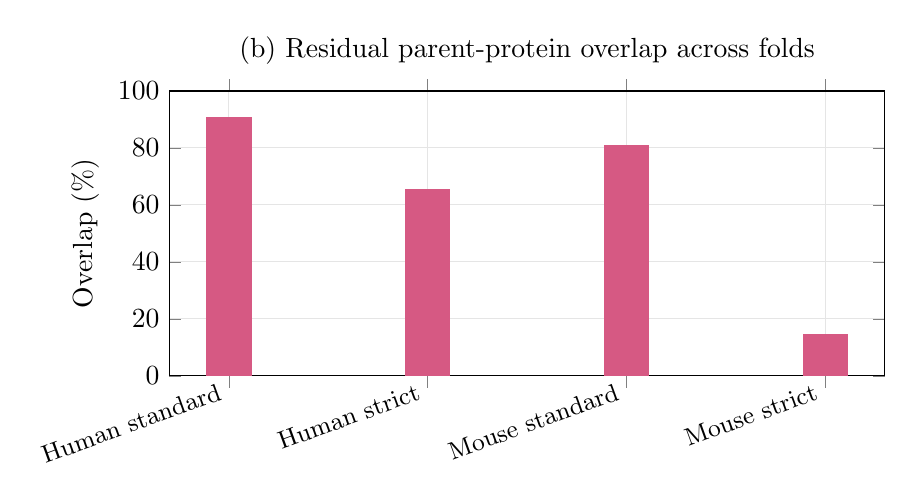
\begin{tikzpicture}
\begin{axis}[
    width=0.88\linewidth,
    height=5.2cm,
    ybar,
    bar width=16pt,
    title={(b) Residual parent-protein overlap across folds},
    ymin=0,ymax=100,
    symbolic x coords={Human standard,Human strict,Mouse standard,Mouse strict},
    xtick=data,
    x tick label style={rotate=20,anchor=east,font=\small},
    ylabel={Overlap (\%)},
    grid=major,
    grid style={gray!20}
]
\addplot+[fill=purple!65,draw=purple!65] coordinates {(Human standard,90.64) (Human strict,65.26) (Mouse standard,80.69) (Mouse strict,14.37)};
\end{axis}
\end{tikzpicture}
\caption{Matched OOF generalization diagnostics. (a) Task-mean globally peptide-disjoint minus matched-standard AUROC by HLA locus or H2 restriction; negative values indicate degradation after peptide separation. (b) Mean fold-level fraction of unique held-out parent proteins also observed during fitting; nonzero values quantify residual protein overlap.}
\label{fig:appendix-gap}
\end{figure}

\section{Strict Architecture Comparison Details}

\begin{table}[htbp]
\centering
\caption{Selected paired AUROC comparisons on the connected-component peptide-disjoint folds. Differences place the first model minus the second; intervals are 10,000-replicate task-bootstrap intervals and \(q\) values are BH-FDR adjusted within the species--metric family.}
\label{tab:appendix-strict-paired}
\scriptsize
\setlength{\tabcolsep}{0.8pt}
\textbf{Human}\par\smallskip
\begin{tabular}{@{}lrrlll@{}}
\toprule
Comparison & Mean & Median & W/T/L & 95\% CI & BH \(q\) \\
\midrule
TissuePMHC $-$ shared & +0.0091 & +0.0095 & 118/0/39 & [0.0067, 0.0116] & $2.27\times10^{-11}$ \\
TissuePMHC $-$ plain & +0.0097 & +0.0081 & 122/0/35 & [0.0076, 0.0119] & $1.36\times10^{-14}$ \\
TissuePMHC $-$ auxiliary & +0.0010 & -0.0008 & 76/1/80 & [-0.0008, 0.0029] & 0.442 \\
TissuePMHC $-$ BLOSUM62 & +0.0440 & -- & 149/0/8 & [0.0392, 0.0489] & $3.43\times10^{-26}$ \\
TissuePMHC $-$ one-hot & +0.0525 & -- & 157/0/0 & [0.0479, 0.0571] & $8.14\times10^{-27}$ \\
Auxiliary $-$ plain & +0.0087 & -- & 144/0/13 & [0.0074, 0.0100] & $3.02\times10^{-23}$ \\
Auxiliary $-$ shared & +0.0081 & -- & 123/0/34 & [0.0058, 0.0103] & $3.30\times10^{-11}$ \\
\bottomrule
\end{tabular}
\par\medskip
\textbf{Mouse}\par\smallskip
\begin{tabular}{@{}lrrlll@{}}
\toprule
Comparison & Mean & Median & W/T/L & 95\% CI & BH \(q\) \\
\midrule
Factorized MMoE $-$ shared & -0.0008 & -0.0018 & 10/0/14 & [-0.0062, 0.0049] & 0.509 \\
Factorized MMoE $-$ BLOSUM62 & +0.0023 & +0.0039 & 14/0/10 & [-0.0052, 0.0091] & 0.509 \\
\bottomrule
\end{tabular}
\end{table}

\begin{table}[htbp]
\centering
\caption{Single-seed stability and ensemble gain under connected-component peptide-disjoint evaluation. Gain is ensemble AUROC minus the mean single-seed AUROC.}
\label{tab:appendix-strict-seeds}
\footnotesize
\setlength{\tabcolsep}{2pt}
\begin{tabular}{llrrrr}
\toprule
Species & Model & Single-seed mean & Seed SD & Ensemble & Gain \\
\midrule
Human & One-hot logistic regression & 0.7127 & 0.0000 & 0.7127 & 0.0000 \\
Human & BLOSUM62 random forest & 0.7193 & 0.0006 & 0.7212 & +0.0019 \\
Human & Shared heads & 0.7313 & 0.0043 & 0.7561 & +0.0248 \\
Human & Plain MLP dual branch & 0.7394 & 0.0043 & 0.7555 & +0.0161 \\
Human & Auxiliary dual branch & 0.7503 & 0.0038 & 0.7642 & +0.0139 \\
Human & TissuePMHC & 0.7505 & 0.0007 & 0.7652 & +0.0147 \\
Mouse & BLOSUM62 random forest & 0.7491 & 0.0012 & 0.7507 & +0.0016 \\
Mouse & Shared heads & 0.7327 & 0.0031 & 0.7538 & +0.0211 \\
Mouse & Factorized MMoE & 0.7211 & 0.0027 & 0.7529 & +0.0318 \\
\bottomrule
\end{tabular}
\end{table}

\clearpage
\section{Frozen General-pMHC Control Details}

\begin{table}[htbp]
\centering
\caption{NetMHCpan binding-affinity (BA) sensitivity analysis. EL and BA ranks are oriented so that larger scores indicate stronger predicted propensity.}
\label{tab:appendix-netmhcpan-el-ba}
\small
\setlength{\tabcolsep}{4pt}
\begin{tabular}{llrrr}
\toprule
Species & Evaluation & BA AUROC & EL AUROC & EL $-$ BA \\
\midrule
Human & Fixed test & 0.6577 & 0.6833 & +0.0256 \\
Human & Train-pool OOF & 0.6559 & 0.6823 & +0.0264 \\
Mouse & Fixed test & 0.6847 & 0.6893 & +0.0046 \\
Mouse & Train-pool OOF & 0.6778 & 0.6802 & +0.0024 \\
\bottomrule
\end{tabular}
\end{table}

\begin{table}[htbp]
\centering
\caption{Cross-fitted incremental stacking with frozen general-pMHC scores. The combined column uses the external score and the corresponding tissue-conditioned model score.}
\label{tab:appendix-general-stacking}
\footnotesize
\setlength{\tabcolsep}{3pt}
\begin{tabular}{lllrr}
\toprule
Species & Protocol & External control & External only & Combined \\
\midrule
Human & Fixed test & MHCflurry presentation & 0.6851 & 0.8453 \\
Human & Fixed test & NetMHCpan EL & 0.6833 & 0.8447 \\
Human & Peptide-disjoint OOF & MHCflurry presentation & 0.6867 & 0.7693 \\
Human & Peptide-disjoint OOF & NetMHCpan EL & 0.6740 & 0.7651 \\
Mouse & Fixed test & MHCflurry presentation & 0.6564 & 0.8565 \\
Mouse & Fixed test & NetMHCpan EL & 0.6893 & 0.8564 \\
Mouse & Peptide-disjoint OOF & MHCflurry presentation & 0.6464 & 0.7564 \\
Mouse & Peptide-disjoint OOF & NetMHCpan EL & 0.6420 & 0.7534 \\
\bottomrule
\end{tabular}
\end{table}
